% Auto-generated by experiments/export_paper_c_latex_artifacts.py
% Do not edit by hand. Regenerate from results/* instead.

% ---- Global count macros (verifiable from results/paper_c_main_findings.txt) ----
\newcommand{\ArimaBetterCount}{7/8}
\newcommand{\LGBMBetterCount}{8/8}
\newcommand{\ArimaGainCollapseCount}{7/8}
\newcommand{\LGBMGainCollapseCount}{8/8}
\newcommand{\LGBMBeatsArimaCount}{7/8}
\newcommand{\LGBMLowerAlphaCount}{8/8}

% ---- Findings extracted from results/paper_c_main_findings.txt ----
% Paper C - Main findings summary (2 stations x 4 horizons = 8 cells)
% ======================================================================
%
% Stations:    Madrid_60, Valencia_Politecnico
% Horizons:    h in {1, 6, 12, 24}
% Evaluation:  Expanding-window rolling-origin CV, 8 folds per (station, horizon)
% Baseline:    Naive persistence
%
% 1. Skill vs persistence
%    - ARIMA improves upon persistence in 7 of 8 (station, horizon) cells
%      (exception: Madrid_60, h=24, where skill_rmse is slightly negative).
%    - LightGBM improves upon persistence in 8 of 8 cells.
%
% 2. Head-to-head model comparison
%    - LightGBM outperforms ARIMA (lower RMSE) in 7 of 8 cells
%      (exception: Madrid_60, h=1, where ARIMA is marginally lower).
%
% 3. Variability / amplitude diagnostics (KGE alpha)
%    - LightGBM exhibits a lower alpha than ARIMA in 8 of 8 cells,
%      indicating stronger amplitude underestimation by the tree ensemble.
%    - ARIMA alpha falls below 0.95 (gain-collapse threshold) in 7 of 8 cells.
%    - LightGBM alpha falls below 0.95 in 8 of 8 cells.
%
% 4. Variance-penalised skill (Skill_VP = Skill_RMSE * min(1, alpha^2))
%    - The apparent RMSE-based gain collapses once the amplitude penalty is
%      applied, most severely at h in {12, 24}.
%
% Verified counts (for LaTeX macros):
%    ArimaBetterCount         = 7/8
%    LGBMBetterCount          = 8/8
%    ArimaGainCollapseCount   = 7/8
%    LGBMGainCollapseCount    = 8/8
%    LGBMBeatsArimaCount      = 7/8
%    LGBMLowerAlphaCount      = 8/8

% Suggested Results/Discussion paragraph (academic English, no over-claim):
%
% Across the two urban PM10 stations and horizons h in {1, 6, 12, 24},
% ARIMA improves upon the persistence baseline in \ArimaBetterCount of
% the station-horizon cells, while LightGBM improves upon it in
% \LGBMBetterCount. In a direct head-to-head comparison, LightGBM
% attains a lower RMSE than ARIMA in \LGBMBeatsArimaCount of the cells.
% The KGE variability ratio alpha is lower for LightGBM than for ARIMA
% in \LGBMLowerAlphaCount of the cells, showing that the tree ensemble
% contracts more strongly toward the conditional mean. Consistently,
% alpha falls below 0.95 -- a gain-collapse regime in which the
% variance-penalised skill Skill_VP lies well under the plain skill
% score -- in \ArimaGainCollapseCount (ARIMA) and \LGBMGainCollapseCount
% (LightGBM) of the cells, with the effect most pronounced at h=12
% and h=24. These findings support the paper's claim that an apparent
% RMSE-based gain can coexist with a marked loss of variability, and
% motivate reporting alpha and Skill_VP alongside RMSE.

% ---- Figures ----
\begin{figure}[t]
\centering
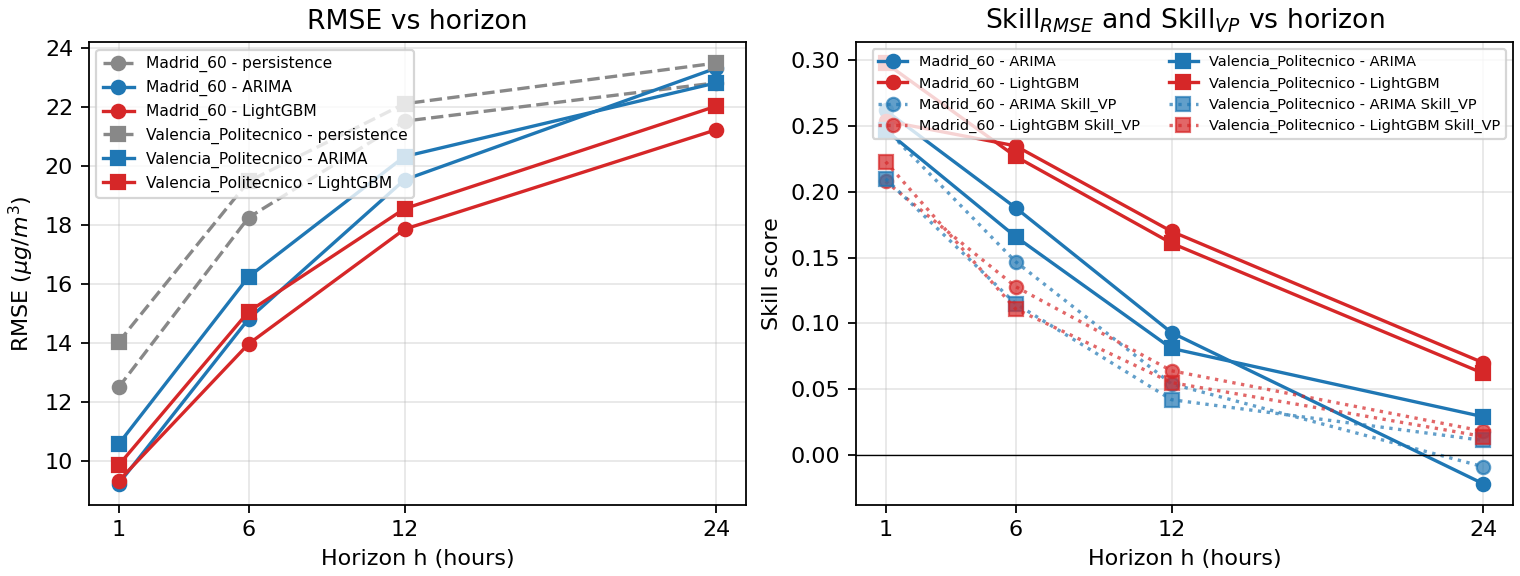
\includegraphics[width=\linewidth]{figures/fig_paper_c_rmse_skill.png}
\caption{RMSE and skill scores as a function of the forecast horizon
$h$ for both stations. Dashed lines report the persistence baseline;
solid lines report ARIMA and LightGBM. The right panel overlays the
variance-penalised skill Skill$^{\mathrm{VP}}$ (dotted), which
collapses toward zero at long horizons despite positive Skill$_{\mathrm{RMSE}}$.}
\label{fig:rmse}
\end{figure}

\begin{figure}[t]
\centering
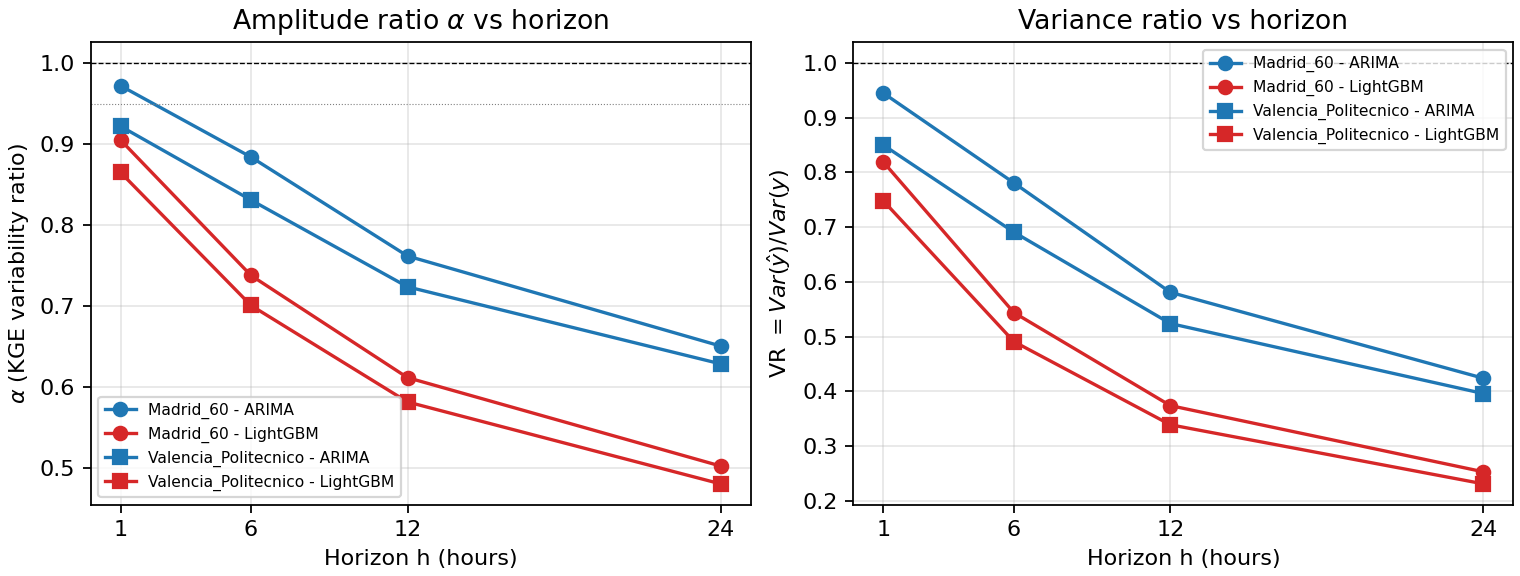
\includegraphics[width=\linewidth]{figures/fig_paper_c_alpha_vr.png}
\caption{KGE variability ratio $\alpha$ (left) and variance ratio
$\mathrm{VR}=\mathrm{Var}(\hat{y})/\mathrm{Var}(y)$ (right) as a
function of the forecast horizon $h$. The dashed reference at $1$
marks perfect amplitude retention; values below it indicate
underdispersion. LightGBM sits systematically below ARIMA on both
panels.}
\label{fig:alpha}
\end{figure}
